\documentclass[a4paper,14pt]{extarticle}
\def\source{/home/osabio/tex/templates}
\input{\source/head.tex}
\yakovlev{113}{Электростатика}
\begin{document}

\begin{figure}[H]
    \centering
    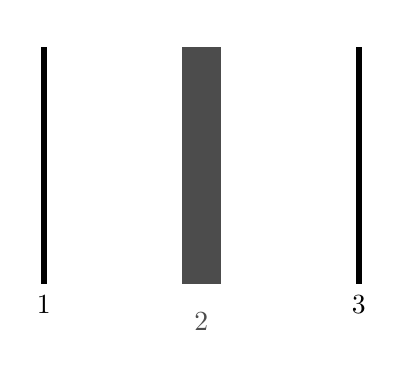
\begin{tikzpicture}
        \draw[line width=2pt] (0,0) node[below] {$1$} -- ++(0,3);
        \draw[line width=0.5cm, black!70] (2,0) node[below] {$2$} -- ++(0,3);
        \draw[line width=2pt] (4,0) node[below] {$3$} -- ++(0,3);
        % \draw[line width=2pt] (6,0) node[below] {$4$} -- ++(0,3);

        % \draw[magenta] (0,3) -- (0,4) -- (4,4) -- (4,3);      
    \end{tikzpicture} 
\end{figure}
Пусть начальная емкость конденсатора $C_0$. Тогда
\begin{equation}
	C_0=\frac{S}{k\cdot4\pi d}
\end{equation}
Расположим медную пластину на расстоянии $l$ внутри конденсатора. Тогда емкость между 1 и 2 будет
\begin{equation}
	C_{12}=\frac{S}{k\cdot4\pi l}
\end{equation}
А между 2 и 3
\begin{equation}
	C_{23}=\frac{S}{k\cdot4\pi (\frac34d-l)}
\end{equation}

Заменим систему эквивалентной, скомпонованной из конденсаторов:
\begin{figure}[H]
    \centering
	\begin{circuitikz}[scale=1.25, every node/.style={scale=1.25}]
		\draw (-2,0) node[anchor=east]{1}
  		to[short, o-*] (0,0)
		% to[] ++(0,2) 
		to[C=$C_{12}$] ++(2,0)
		to ++(0,-2)
		to[C=$C_{23}$] ++(-2,0);
		\draw (-2,-2) node[anchor=east]{3}
  		to[short, o-*] ++(2,0);
	\end{circuitikz}
\end{figure}
Общая емкость конденсаторов  $C_{12}$ и $C_{23}$
\begin{equation}
	\frac{1}{C}=\frac{1}{C_{12}}+\frac{1}{C_{23}}=
	\frac{1}{S}\left[
		{k\cdot4\pi (\frac34d-l)}+
		{k\cdot4\pi l}
	\right]=\frac{k\cdot 3\pi d}{S}
\end{equation}
То есть
\begin{equation}
	C=\frac{S}{k\cdot 3\pi d}=\frac43C_0
\end{equation}
\begin{equation}
	C-C_0=\frac13C_0=200 \text{ Пф}
\end{equation}
Как видно, положение листа $l$ не влияет на ответ (емкость увеличивается на треть). Важно, чтобы лист оставался параллелен обкладкам, тогда будут верны использованные при выводе формулы плоского конденсатора.

\end{document}